% ==================================================
\chapter{Results}\label{chap:Results}
% ==================================================

% --------------------------
\section{User Feedback - Usability Study}
% --------------------------



A total of 15 participants from various disciplines including Natural Sciences, Social Sciences, Life Sciences, and Computer Science evaluated Scholar Plot. We asked each participant to review the interface and complete an online survey. Special care was taken to ensure that the participants had correct understanding about the visualization component before they began rating. The participants answered the questions on a Likert scale from 1 to 5 with 1 being strongly disagree and 5 being strongly agree.

Figure \ref{fig:UserStudy} illustrates the mean evaluation for each visualization component. Accuracy, usability, and understandability of Scholar Plot scored the highest $(\mu = 4.2)$ as it is very intuitive and can be used with minimal assistance. The highest positive feedback we received from many of the participants was the visual scheme of Scholar Plot. Another observation is that the participants agree to use Scholar Plot to evaluate themselves $(\mu = 4.1)$. They suggested that Scholar Plot can be improved by adding more funding agencies. Overall, this evaluation indicated that Scholar Plot is a user-friendly tool that complements the CV which can be used to review a scholar's accomplishments. The survey has been approved by the University of Houston Institutional Review Board (IRB).

 \begin{figure}[!htb]
  \centering
  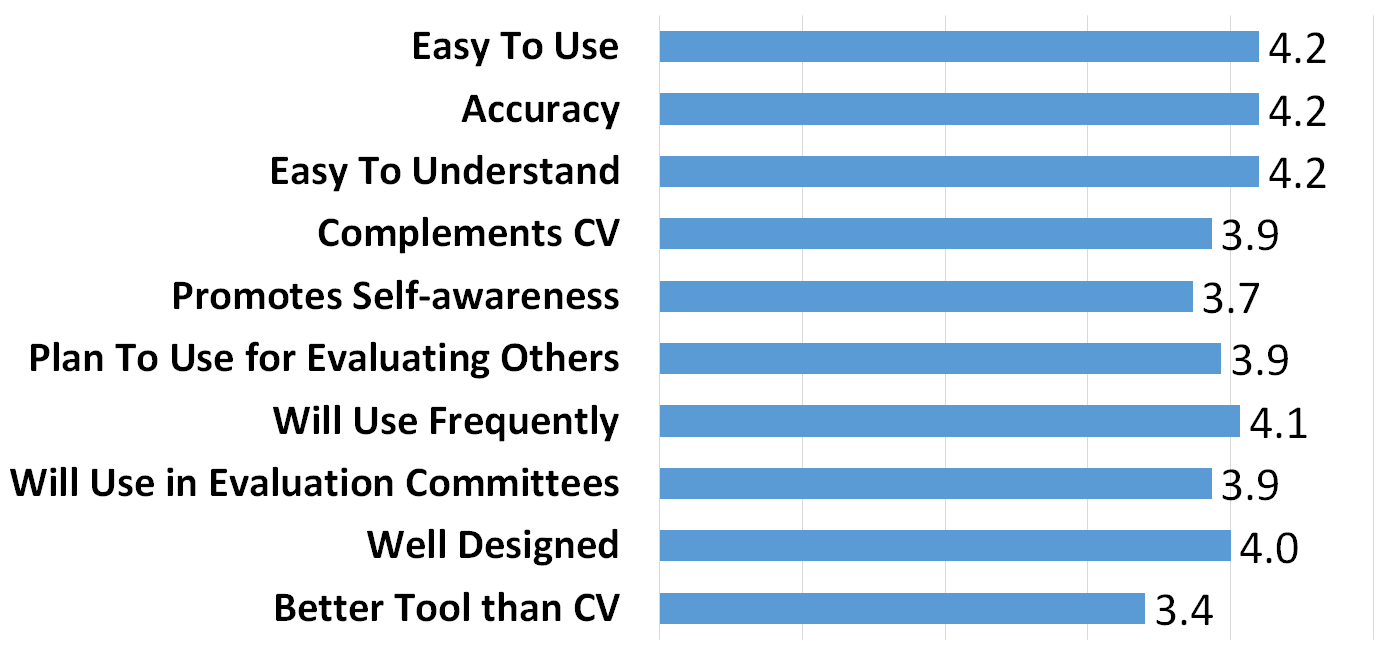
\includegraphics[width=\textwidth]{figures/fig_survey_chart}
%  \vspace{-3ex}
  \caption{Mean evaluation of Scholar Plot. A total of $n=15$ participants evaluated the survey.}
  \label{fig:UserStudy}
\end{figure}



% --------------------------
\section{User Feedback - Focus Group}
% --------------------------

We ran a focus group with 10 Principal Investigators and their post doctoral students at Northwestern University. The participant set included biologists, physicists, computer scientists, and social scientists. The focus group's suggestions are synopsized as follows:
\begin{description}
\item [Interface team science information.] Participants wanted to see the number and intensity of collaborations for the depicted scholar.
\item [Summarize highly cited papers.] Participants wanted to see explicitly in a side panel the scholar's most popular papers.
\item [Interface journal profile.] Participants wanted to see the specific journals where the scholar publishes most often and their impact factors.
\end{description}

The participants believed that accessorizing the central publication graph with this additional information would support deeper instant comprehension without compromising the elegance of Scholar Plot's compact visual representation. Specifically, this additional interface would reveal the collaborative nature of the scholar's work, give hints if s/he is a regular in specific disciplinary journals or if publishes in a variety of journals (interdisciplinarity), and give the rank of these journals. % All this information can also be gleaned by rolling the mouse over the publication graph, reading the tooltips, and summarizing it in panels under the graph. However, renders such manual investigation unnecessary.

\begin{figure}[H]
    \centering
    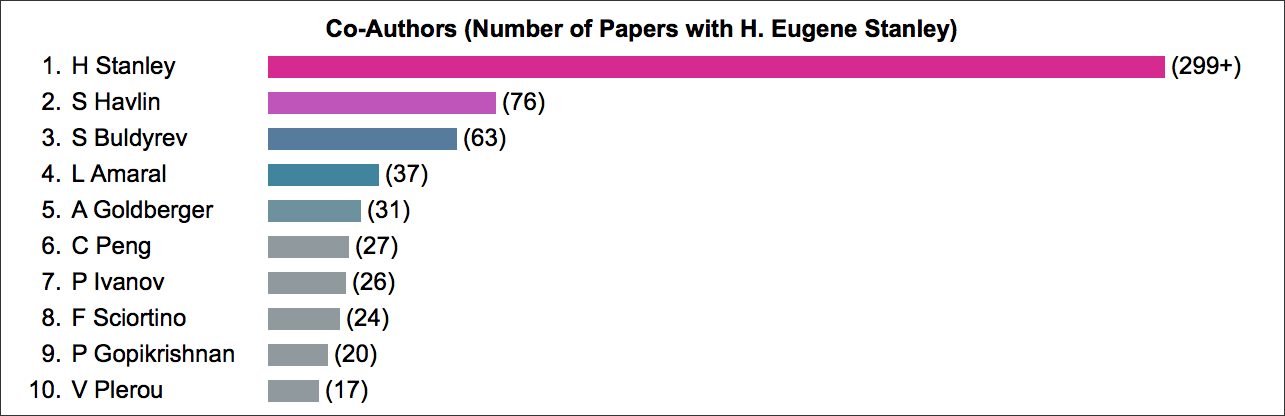
\includegraphics[width=\textwidth]{figures/fig_panel1-N}
    \caption{Panel listing the top collaborators with the selected scholar ranked by the count of the number of publications collaborated.}
    \label{fig:panel1}
\end{figure}

\begin{figure}[H]
    \centering
    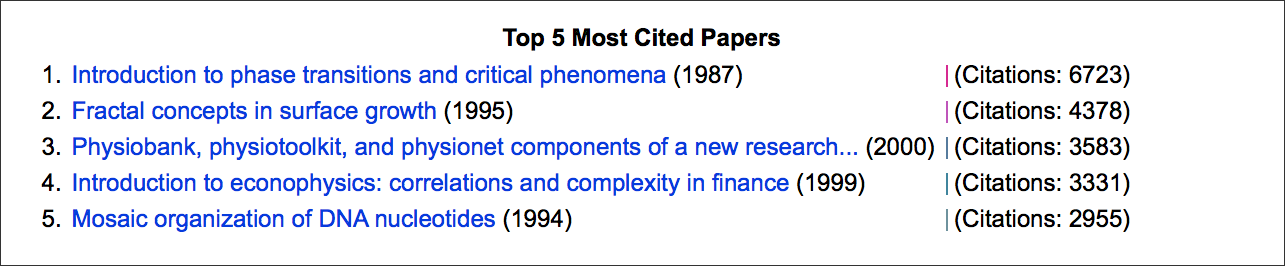
\includegraphics[width=\textwidth]{figures/fig_panel3-N}
    \caption{Panel highlighting the top 5 cited papers of the selected scholar.}
    \label{fig:panel3}
\end{figure}

\begin{figure}[H]
    \centering
    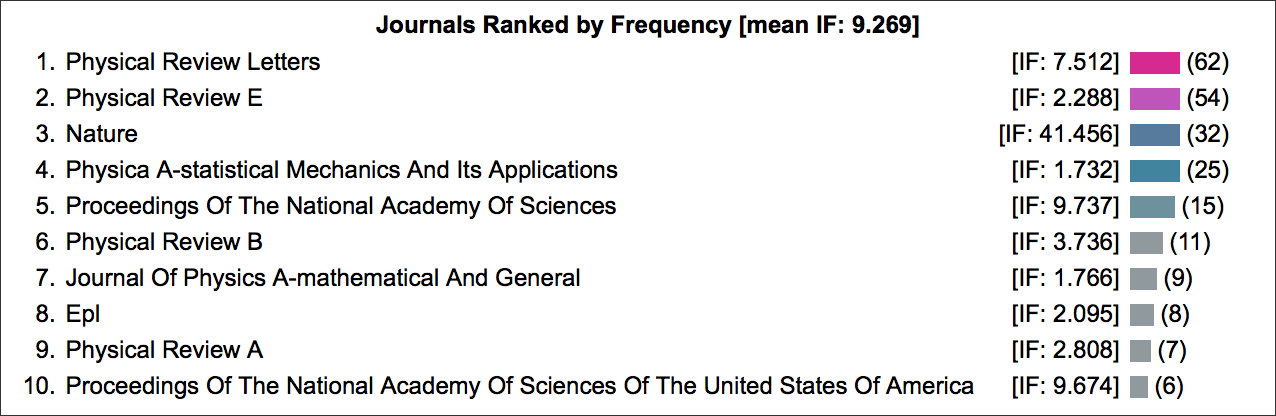
\includegraphics[width=\textwidth]{figures/fig_panel2-N}
    \caption{Panel displaying the top journals ranked by the frequency of publication.}
    \label{fig:panel2}
\end{figure}

\begin{figure}[H]
    \centering
    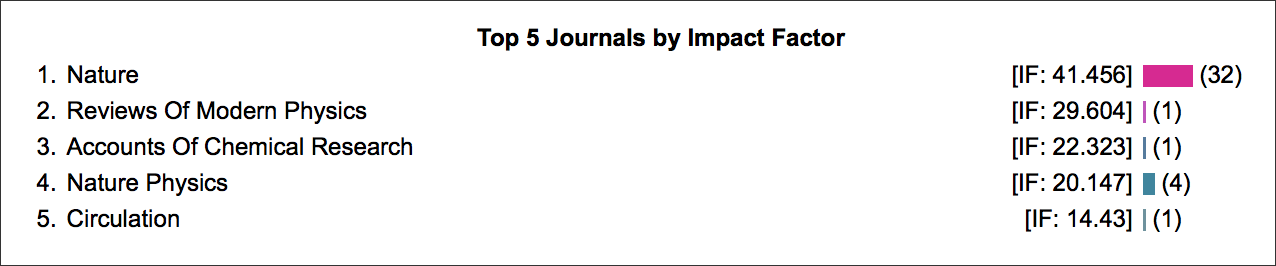
\includegraphics[width=\textwidth]{figures/fig_panel4-N}
    \caption{Panel showing the top 5 journals where the selected scholar published ranked by the impact factor.}
    \label{fig:panel4}
\end{figure}




% --------------------------
\section{Global and Local Bias Correction}
% --------------------------
%Academic Garden reveals that people look relatively important locally in low ranking departments, like University of Houston, (See Figure: \ref{fig:uh-local}) but there are not so important in the global scheme of visualization (See Figure: \ref{fig:uh-global}). The opposite is true for very high ranking departments, like MIT, where many people might look unimportant locally (See Figure: \ref{fig:mit-local}) because of a couple of outstanding people within the department even though they are quite good in their discipline (See Figure: \ref{fig:mit-global}).

Academic Garden reveals that some people stand out locally in low ranking departments such as the University of Houston (See Figure: \ref{fig:uh-local}) but are ordinary in the global scheme of visualization (See Figure: \ref{fig:uh-global}). The opposite is true for very high-ranking departments such as Massachusetts Institute of Technology (MIT) where, because of a couple of outstanding people, others may appear unimportant locally (See Figure: \ref{fig:mit-local}) though they are quite good in their discipline (See Figure: \ref{fig:uh-global}).

Providing both visualization schemes to the user makes Academic Garden a useful tool for every academic department no matter how they are ranked. 
Rather than a log scale, which would unjustifiably elevate the lowest performing faculty and not adequate acknowledge the merit of the highest performing faculty, the local scheme displays a department using a linear scale. The local scale is dynamic and is adjusted to the maximum citation count of the department.

The global scale has two linear sections. The top section has a fixed minimum of 20,001 and a fixed maximum of 300,000, which is larger than the highest number of citations in the global dataset. The bottom section has a fixed range of 0-20,000 citations, which represents the $90^{\text{th}}$ percentile of the global dataset. The larger height of the bottom section displays the $90^{\text{th}}$ percentile of faculty vertically across Academic Garden instead of compressing it to the very bottom.

\begin{figure}[H]
    \centering
    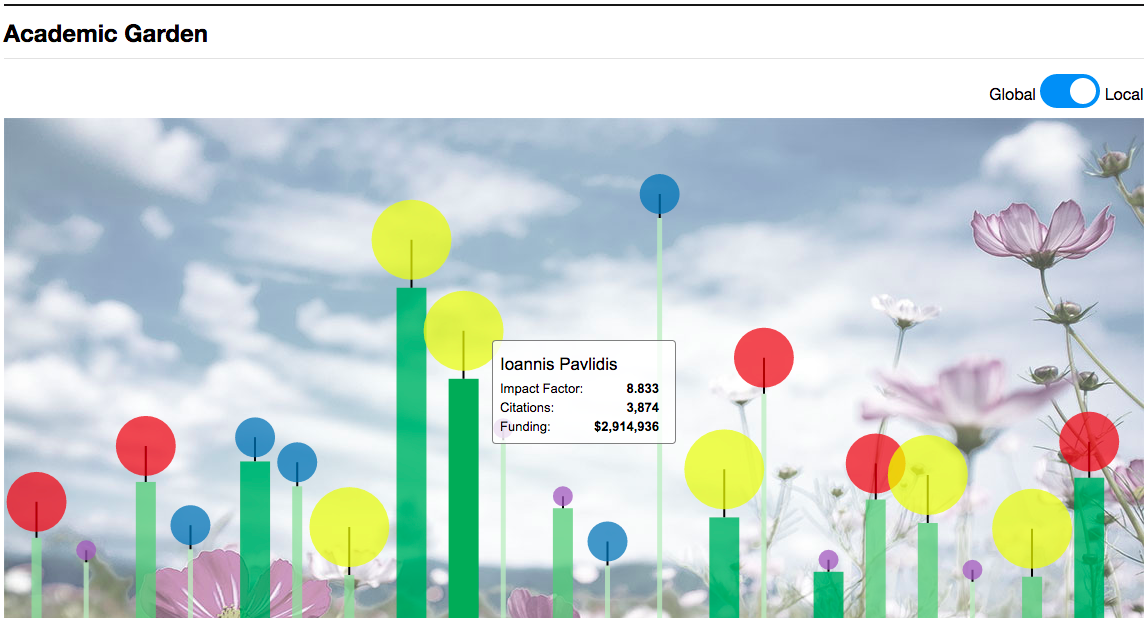
\includegraphics[width=0.9\textwidth]{figures/fig-UH-Local}
    \caption{Local Scale: Department of Computer Science at the University of Houston.}
    \label{fig:uh-local}
\end{figure}

\begin{figure}[H]
    \centering
    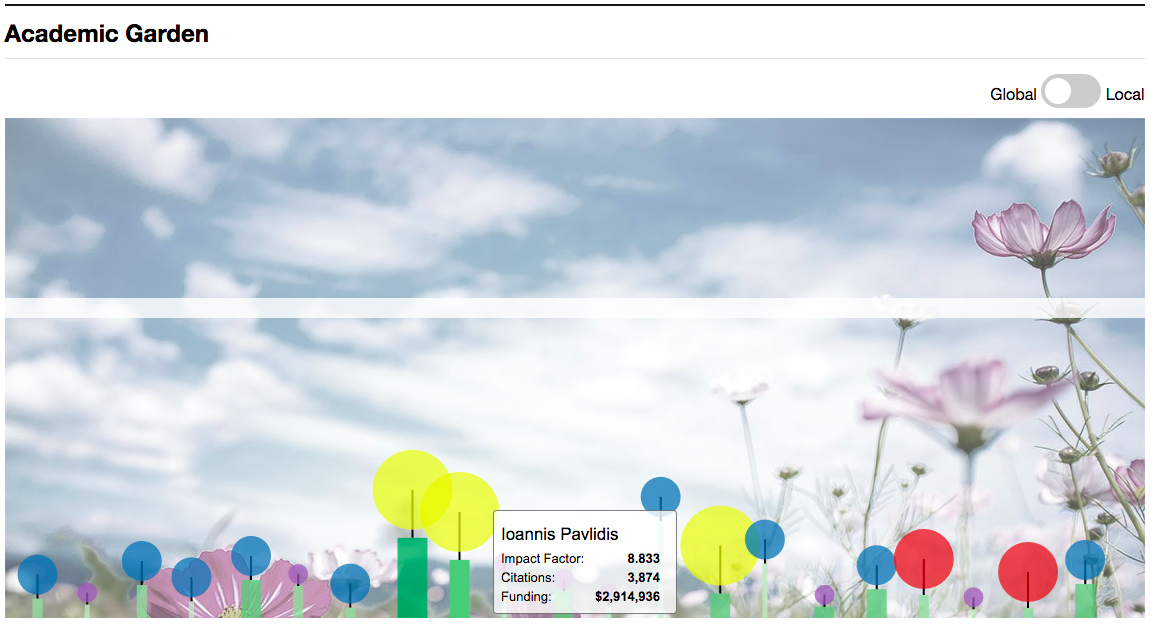
\includegraphics[width=0.9\textwidth]{figures/fig-UH-Global}
    \caption{Global Scale: Department of Computer Science at the University of Houston.}
    \label{fig:uh-global}
\end{figure}



\begin{figure}[H]
    \centering
    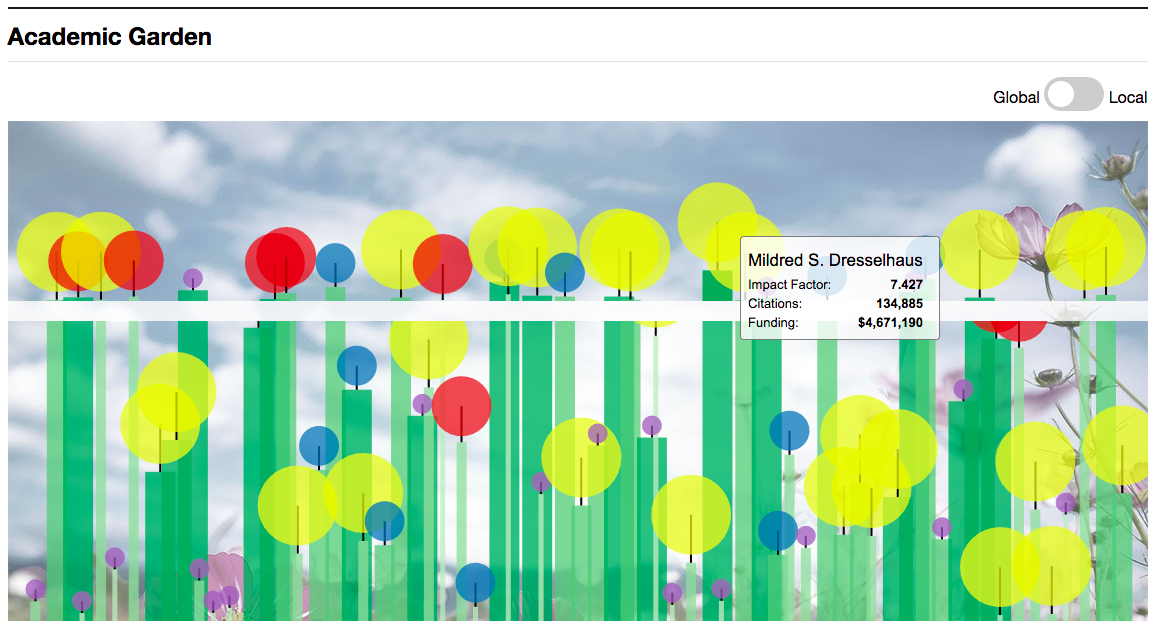
\includegraphics[width=0.9\textwidth]{figures/fig-MIT-Global}
    \caption{Global Scale: Department of Computer Science at the MIT.}
    \label{fig:mit-global}
\end{figure}

\begin{figure}[H]
    \centering
    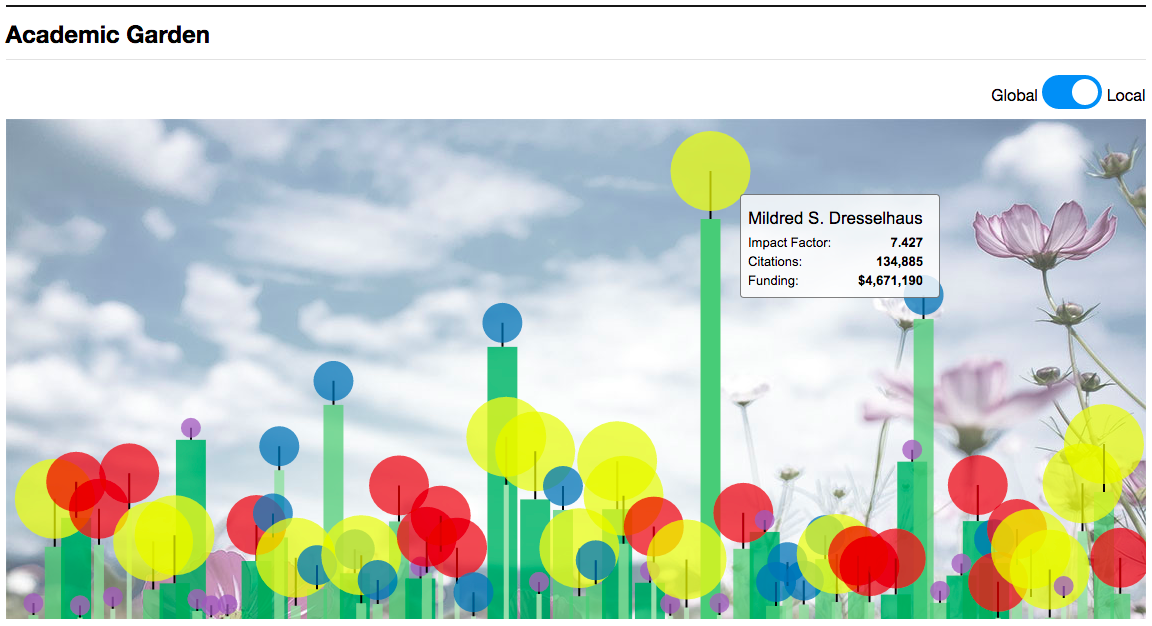
\includegraphics[width=0.9\textwidth]{figures/fig-MIT-Local}
    \caption{Local Scale: Department of Computer Science at the MIT.}
    \label{fig:mit-local}
\end{figure}





% --------------------------
\section{Data Analysis}
% --------------------------
For the validation of our design choices of Academic Garden, I used chaired faculty as the ground truth. An Endowed Chair is considered a prestigious award in the United States. I ran linear models in R software \cite{R:The81:online} to understand the validity of the design with respect to Endowed Chairs. 

The data was collected in July 2016. This included total 14 different universities. The data consists of $( n = 248 )$ faculty from Computer Science and $( n = 152 )$ from Biology from the top 10 schools according the US News Report 2015 \cite{usnews}. The data of chaired faculty consists of $( n = 61 )$ chaired professors from Computer Science and  $( n = 32 )$ from Biology in top 10 schools.


% For tables use
\begin{table*}
\centering
% table caption is above the table
\caption{The list of institutes in Computer Science by rank sourced from U.S. News \cite{usnews}.}
\label{tab:1}       % Give a unique label
% For LaTeX tables use
\begin{tabular}{rl}
\hline\noalign{\smallskip}
Rank & Department of Computer Science \\
\noalign{\smallskip}\hline\noalign{\smallskip}
1 & University of California, Berkeley \\
1 & Carnegie Mellon University \\
1 & Massachusetts Institute of Technology \\
1 & Stanford University \\
5 & University of Illinois at Urbana-Champaign \\
6 & Cornell University \\
6 & University of Washington \\
8 & Princeton University \\
9 & Georgia Institute of Technology \\
10 & University of Texas, Austin  \\
\noalign{\smallskip}\hline
\end{tabular}
\end{table*}



% For tables use
\begin{table*}
\centering
% table caption is above the table
\caption{The list of institutes in Biology by rank sourced from U.S. News \cite{usnews}.}
\label{tab:}       % Give a unique label
% For LaTeX tables use
\begin{tabular}{rl}
\hline\noalign{\smallskip}
Rank & Department of Biology  \\
\noalign{\smallskip}\hline\noalign{\smallskip}
1 & Harvard University \\
1 & Massachusetts Institute of Technology \\
1 & Stanford University \\
4 & University of California, Berkeley \\
5 & California Institute of Technology \\
5 & Johns Hopkins University \\
7 & University of California San Francisco \\
7 & Yale University \\
9 & Princeton University \\
10 & Cornell University \\

\noalign{\smallskip}\hline
\end{tabular}
\end{table*}

The three criteria we used in the Academic Garden are citations, impact factor, and funding. We computed the quartiles for these three criteria based on the local department faculty, as well as the global scale considering all the faculty from the same discipline. We obtained the discipline information from the Classification of Instructional Programs (CIP) codes from The National Center for Education Statistics designed the Classification of Instructional Program \cite{CIPus76:online}.


For each faculty, we computed the quartile to which he belongs to for each of the three criteria in the local and global scales. We also computed a variable to determine if a faculty belongs to either one of the top 3 criteria.
For Computer Science, this variable significantly predicts chaired faculty ( p $<$ 0.05 ) i.e, we can predict a faculty is chaired if he belongs to the top quartile locally in either of the three criteria.

The values are seen in Figures \ref{fig:CS-Local-Quartile}. In this model, quartiles are calculated with respect to the department which the faculty belongs to.

 \begin{figure}
  \centering
  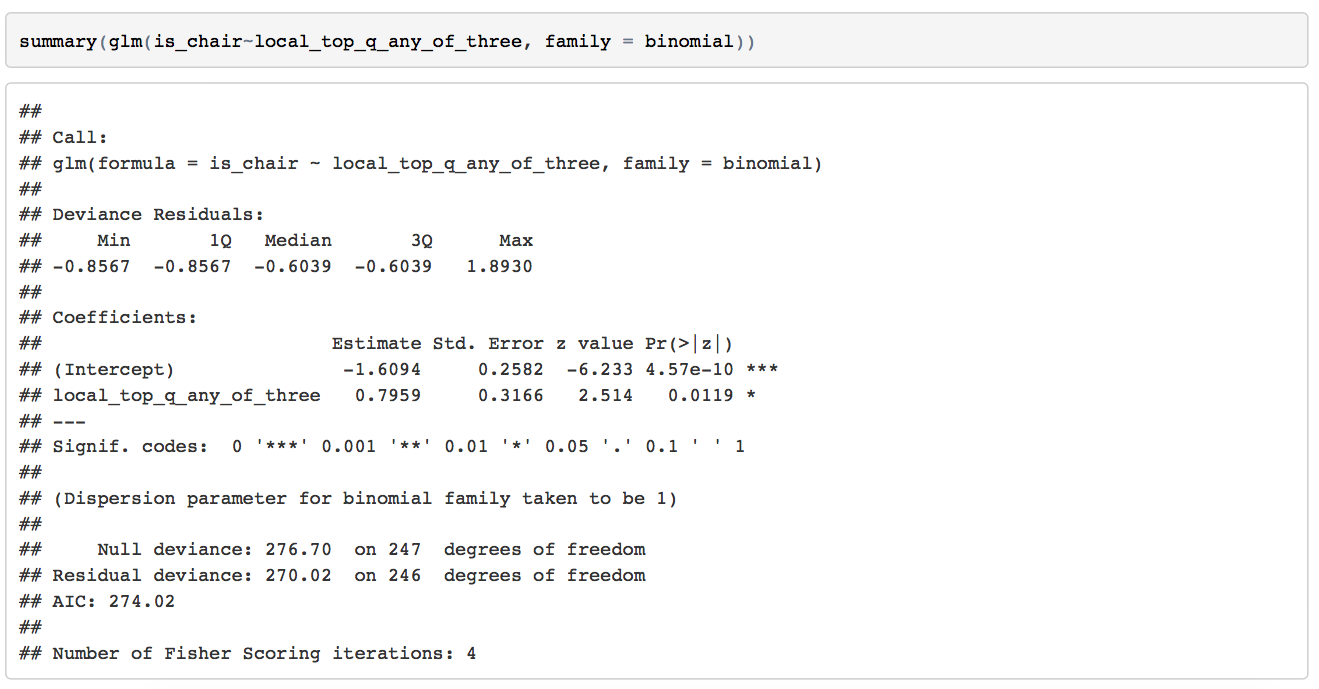
\includegraphics[width=\textwidth]{figures/CS-Local-Quartile}
%  \vspace{-3ex}
  \caption{Screenshot of a result of Linear Model in R.}
  \label{fig:CS-Local-Quartile}
\end{figure}

All three criteria can be considered as separate factors. In computer science, citations are highly significant ( p $<$ 0.001 ) while the mean impact factor is not significant. This is because computer science faculty do not publish as much in journals. The funding is also not significant because our funding sources (NSF/NIH/NASA) do not include most funding sources which computer science faculty obtains funding, for example, DoD (United States Department of Defense) and DHS (United States Department of Homeland Security).

However, in the case of Biology, the funding quartile is significant ( p $<$ 0.01 ) because of the funding dataset includes NSF, NIH from where most the Biology grants are from (Figures: \ref{fig:BIO-local-funding}). Also, the Impact Factor quartile is significant ( p $<$ 0.05 ) because they publish more in journals.

 \begin{figure}
  \centering
  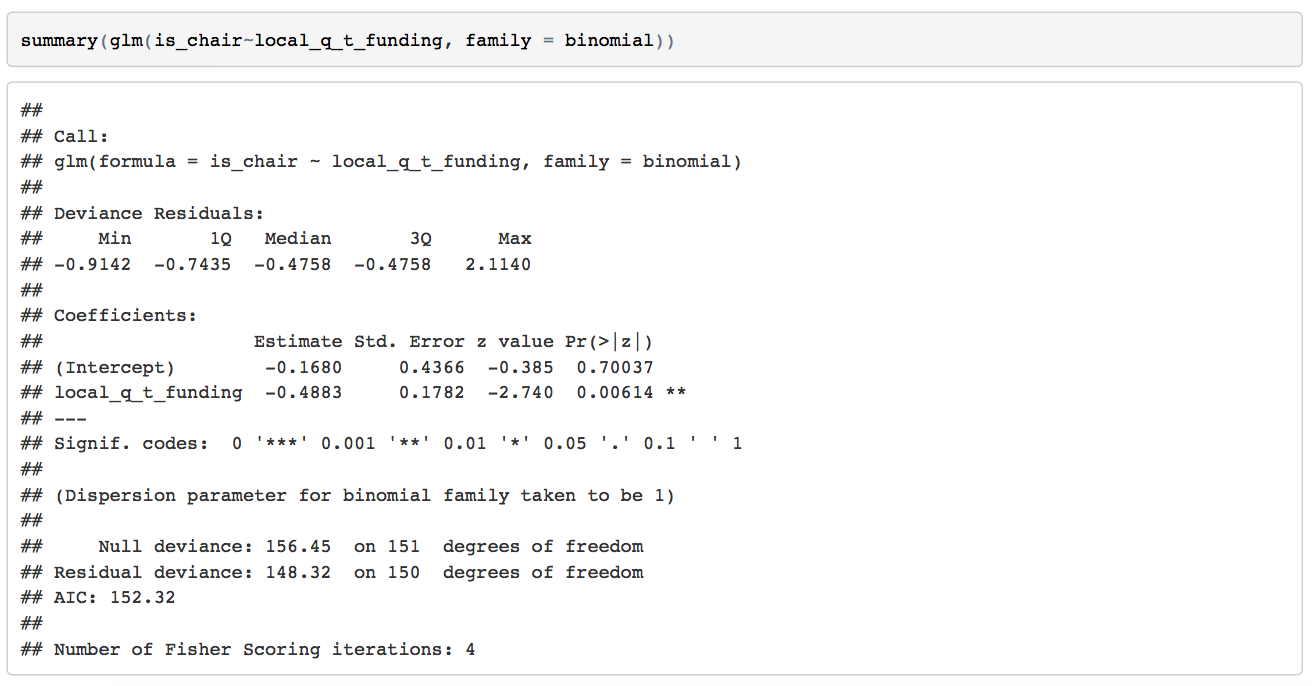
\includegraphics[width=\textwidth]{figures/BIO-local-funding}
%  \vspace{-3ex}
  \caption{Screenshot of a result of Linear Model in R.}
  \label{fig:BIO-local-funding}
\end{figure}

According to the results of linear model, the data analysis validates the design choice of the three criteria for the visualization, and it is exactly mirroring visualization with quartiles values.




%1.	Biologists publish less than computer scientists and have more authors per paper. The mean number of publications per year in Biology (5.21) is significantly lower (t-test, p < 0.01) than the respective mean in Computer Science (8.58). In contrast, the mean number of coauthors in Biology publications (5.57) is significantly higher (t-test, p < 0.01) than the respective mean in Computer Science (4.71).

%2.	Biologists publish mainly in journals, while Computer Scientists less so. The percentage of journal publications is significantly higher (t-test, p < 0.01) in Biology (73.36\%) with respect to Computer Science (19.83\%).

%3.	Biology's elite dominates publications in their top journals a lot more than the Computer Science elite does in theirs. Within the ranked set of all Biology journals, our Biology faculty sample publishes in the top 11\%. In contrast, within the ranked set of all Computer Science journals, our Computer Science faculty sample publishes in the top 24\%. 

%4.	There is significant correlation between the citations obtained per year versus the number of publications produced per year in both disciplines, with Biology (p < 0.01,  = 81.15, R2 = 0.54) having a steeper slope than Computer Science (p = 0.01,  = 40.81, R2 = 0.19). The latter suggests that Biology has a tendency for higher mean citation-impact per article than Computer Science.


